\documentclass[11pt,a4paper]{article}
\usepackage[
    left=0.73in,
    right=0.73in,
    top=.8in,
    bottom=.50in,
    paperheight=11in,
    paperwidth=8.5in
]{geometry}

\usepackage{graphicx}
\usepackage{float}

\begin{document}
% Cover Page
\pagenumbering{gobble}
\begin{center}
\textbf{
    \Large{ECE 543: Introduction to Digital Systems}
    \\~\\
    \large{Instructor: Bessam Zuhair Al Jewad, Ph.D.}
    \\[1.25in]
    \LARGE{Prelab \#7: Data Storage Registers}
    \\[0.62in]
    \large{Prepared for Himadri Basu (TA)\\~\\By Christopher Chin}
    \\[1.25in]
    \LARGE{Section 6}
    \\[1.25in]
    \Large{Department of Electrical and Computer Engineering\\
           University of New Hampshire}
    \\[1.25in]
    \Large{\today}
}
\end{center}
\clearpage
\pagenumbering{arabic}

% TOC
\tableofcontents
\pagebreak

% Pages
\section{Introduction}
\section{Equipment Required}
\begin{itemize}
    \item Global Specialties Design and Prototyping PB-505
    \item Wire leads
    \item 74175 TTL Quad D Positive Edge-Triggered Flip-Flop Integrated Circuit (1)
\end{itemize}
\section{Parallel Latch Register}
\subsection{Wiring Diagram}
\begin{figure}[H]
    \centering
    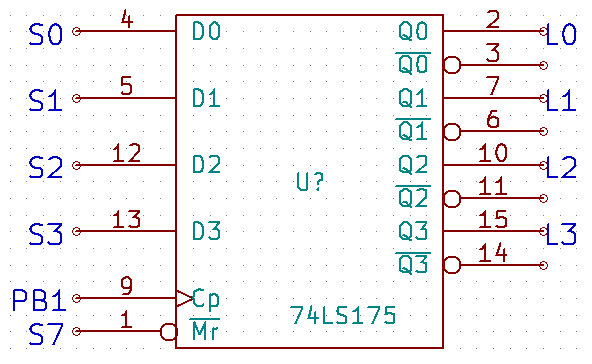
\includegraphics[width=5in]{parallel.png}
    \caption{Parallel Latch Register}
\end{figure}
\subsection{Truth Table}
\begin{tabular}{| c | c | c | c |}
    \hline CLR & CLK & $S_3S_2S_1S_0$ & $Q_3Q_2Q_1Q_0$ \\
    \hline 0 & 1 & XXXX & 0000 \\
    \hline 1 & 1 & 0000 & 0000 \\
    \hline 1 & 1 & 0001 & 0001 \\
    \hline 1 & 1 & 0010 & 0010 \\
    \hline 1 & 1 & 0011 & 0011 \\
    \hline 1 & 1 & 1111 & 1111 \\
    \hline
\end{tabular}
\section{Right Shift Register}
\subsection{Wiring Diagram}
\begin{figure}[H]
    \centering
    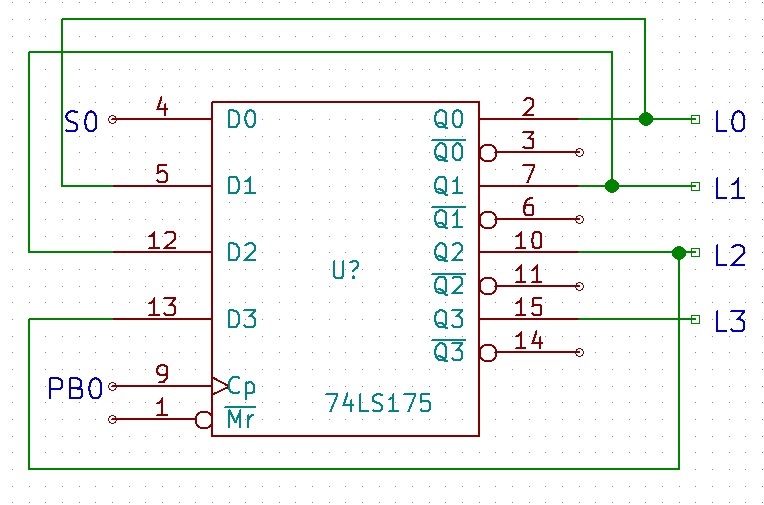
\includegraphics[width=5in]{right_shift.png}
    \caption{Right Shift Register}
\end{figure}
\subsection{Truth Table}
\begin{tabular}{| c | c | c | c |}
    \hline CLR & CLK & $S_0$ & $Q_3Q_2Q_1Q_0$ \\
    \hline 1 & 1 & 1 & 0001 \\
    \hline 1 & 1 & 0 & 0010 \\
    \hline 1 & 1 & 0 & 0100 \\
    \hline 1 & 1 & 0 & 1000 \\
    \hline
\end{tabular}
\section{Left Shift Register}
\subsection{Wiring Diagram}
\begin{figure}[H]
    \centering
    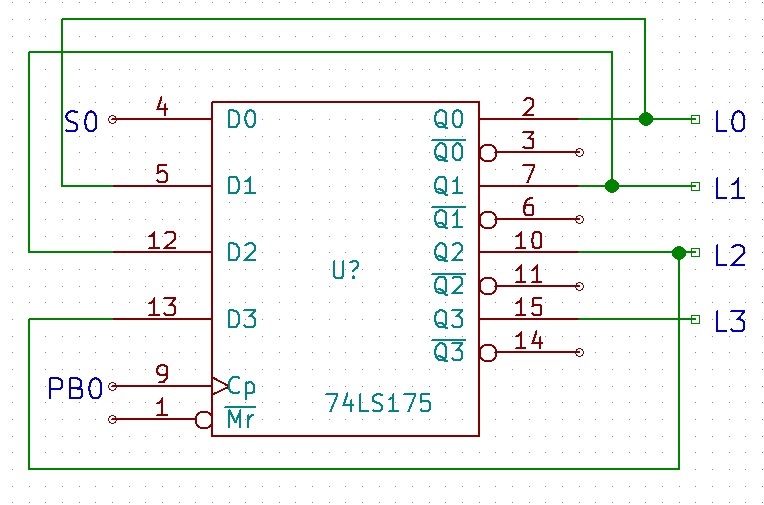
\includegraphics[width=5in]{right_shift.png}
    \caption{Left Shift Register}
\end{figure}
\subsection{Truth Table}
\begin{tabular}{| c | c | c | c |}
    \hline CLR & CLK & $S_0$ & $Q_3Q_2Q_1Q_0$ \\
    \hline 1 & 1 & 1 & 1000 \\
    \hline 1 & 1 & 0 & 0100 \\
    \hline 1 & 1 & 0 & 0010 \\
    \hline 1 & 1 & 0 & 0001 \\
    \hline
\end{tabular}
\section{References}
Ronald J. Tocci et al. 2011. Digital Systems: Principles and Applications, 11\textsuperscript{th} Ed.

\end{document}
